\subsubsection{MapComponent}
Το δεύτερο είναι το Map Component και είναι ένα Component το οποίο προσφέρει ένα προ-ρυθμισμένο Chart από την βιβλιοθήκη Highcharts Highmaps και προσφέρει μια εύκολη διεπαφή για την αλληλεπίδραση και εμφάνιση δεδομένων σε αυτόν τον χάρτη όπως φαίνεται στο σχήμα \ref{layout:mapcomponent}. Κάθε φορά που ο δείκτης του ποντικιού περνάει πάνω απο μια χώρα εμφανίζεται ενα tooltip που γράφει το όνομα της χώρας και σε πόσες ταινίες έχει συμμετάσχει αυτή η χώρα. Όταν πατηθεί μια χώρα θα επιλεγεί εκτός αν ήταν ήδη επιλεγμένη που τότε θα σταματήσει να είναι επιλεγμένη και θα αλλάξει η διεύθυνση όπως φαίνεται στον κώδικα στο σχήμα \ref{code:map_urlchanger}.
\begin{figure}[H]
  \centering
  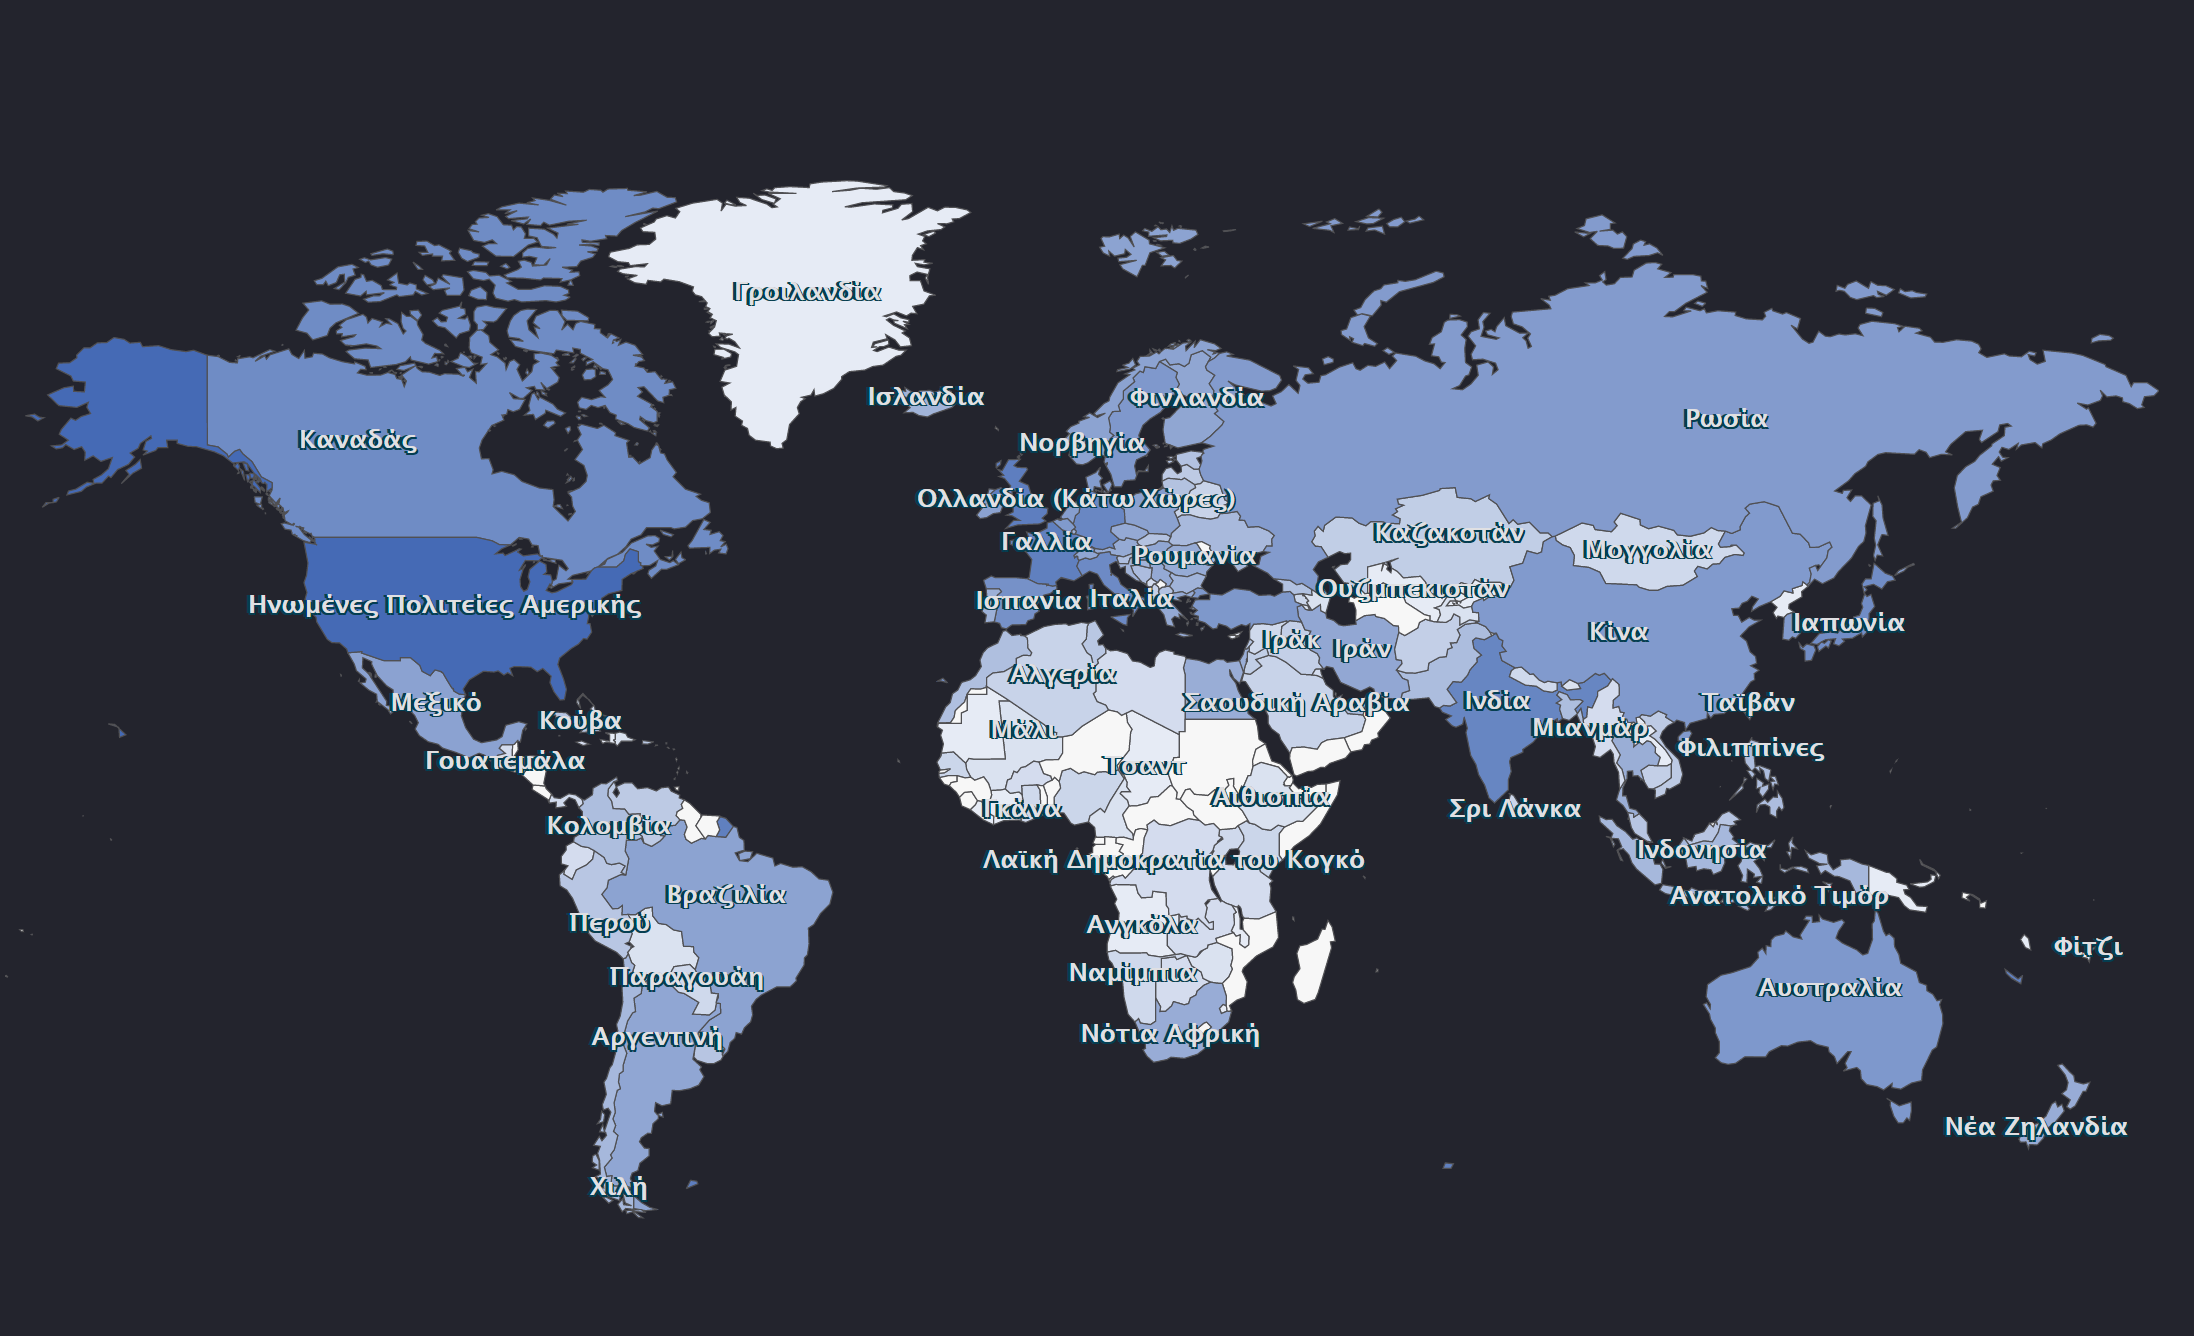
\includegraphics[width=140mm]{Chapters/5 - Architecture/Client/Images/world_map.PNG}
  \caption{Map Component}
  \label{layout:mapcomponent}
\end{figure}

\begin{figure}[H]
    \begin{TypeScriptcode}
countrySelected = (data: ICountryData) => {
  this.props.history.push(AppUtils.|$\textbf{generateNavigationLink}$|({id: data._id, name: data.name, iso31661: data.iso31661, movies: []} as IProductionCountry))
}
countryUnselected = () => {
  this.props.history.push(`/app`)
}
    \end{TypeScriptcode}
    \caption{Αλγόριθμος αλλαγής διεύθυνσης απο το Map Component.}
   \label{code:map_urlchanger}
\end{figure}